\section{Results}\label{sec:results}

\begin{table}[t]
\centering
\caption{\textbf{Fine-tuned Phi-3.5 is best on every metric.} All systems on the full 2024 test set (36{,}325 CVEs). Values are percentages except score MAE. $\pm$ gives the half-width of the 95\% bootstrap interval. Bold marks the best value in each column. The TF-IDF direct systems share one ridge regression, so their score MAE is identical.}
\label{tab:main}
\small
\setlength{\tabcolsep}{4pt}
\begin{tabular}{lcccccc}
\toprule
 & \multicolumn{2}{c}{Severity} & CWE & Score & \multicolumn{2}{c}{Vector} \\
\cmidrule(lr){2-3}\cmidrule(lr){6-7}
System & Acc. & Macro-F1 & Acc. & MAE $\downarrow$ & Partial & Exact \\
\midrule
TF-IDF + LR, direct & 67.1\,{\scriptsize$\pm$0.5} & 47.9\,{\scriptsize$\pm$0.6} & 67.2\,{\scriptsize$\pm$0.5} & 0.98\,{\scriptsize$\pm$0.01} & 86.9\,{\scriptsize$\pm$0.2} & 44.1\,{\scriptsize$\pm$0.5} \\
TF-IDF + LR, formula & 67.1\,{\scriptsize$\pm$0.5} & 51.6\,{\scriptsize$\pm$0.8} & 67.2\,{\scriptsize$\pm$0.5} & 0.94\,{\scriptsize$\pm$0.01} & 86.9\,{\scriptsize$\pm$0.2} & 44.1\,{\scriptsize$\pm$0.5} \\
TF-IDF + LR balanced, direct & 65.7\,{\scriptsize$\pm$0.5} & 51.9\,{\scriptsize$\pm$0.8} & 67.2\,{\scriptsize$\pm$0.5} & 0.98\,{\scriptsize$\pm$0.01} & 86.0\,{\scriptsize$\pm$0.2} & 40.5\,{\scriptsize$\pm$0.5} \\
TF-IDF + LR balanced, formula & 67.1\,{\scriptsize$\pm$0.5} & 53.9\,{\scriptsize$\pm$0.9} & 67.2\,{\scriptsize$\pm$0.5} & 0.98\,{\scriptsize$\pm$0.01} & 86.0\,{\scriptsize$\pm$0.2} & 40.5\,{\scriptsize$\pm$0.5} \\
TF-IDF + RF, direct & 66.9\,{\scriptsize$\pm$0.5} & 47.1\,{\scriptsize$\pm$0.6} & 65.2\,{\scriptsize$\pm$0.5} & 0.98\,{\scriptsize$\pm$0.01} & 86.1\,{\scriptsize$\pm$0.2} & 41.8\,{\scriptsize$\pm$0.5} \\
TF-IDF + RF, formula & 64.0\,{\scriptsize$\pm$0.5} & 47.8\,{\scriptsize$\pm$0.6} & 65.2\,{\scriptsize$\pm$0.5} & 1.03\,{\scriptsize$\pm$0.01} & 86.1\,{\scriptsize$\pm$0.2} & 41.8\,{\scriptsize$\pm$0.5} \\
Phi-3.5 + LoRA, direct & \textbf{69.9}\,{\scriptsize$\pm$0.5} & \textbf{55.7}\,{\scriptsize$\pm$0.9} & \textbf{70.9}\,{\scriptsize$\pm$0.5} & \textbf{0.85}\,{\scriptsize$\pm$0.01} & \textbf{87.9}\,{\scriptsize$\pm$0.2} & \textbf{48.8}\,{\scriptsize$\pm$0.5} \\
Phi-3.5 + LoRA, formula & \textbf{69.9}\,{\scriptsize$\pm$0.5} & \textbf{55.7}\,{\scriptsize$\pm$0.9} & \textbf{70.9}\,{\scriptsize$\pm$0.5} & \textbf{0.85}\,{\scriptsize$\pm$0.01} & \textbf{87.9}\,{\scriptsize$\pm$0.2} & \textbf{48.8}\,{\scriptsize$\pm$0.5} \\
\bottomrule
\end{tabular}
\end{table}


\subsection{Main Results}
Table~\ref{tab:main} reports every system on the \nTest{} test CVEs, and the fine-tuned Phi-3.5 model leads on every metric, with \nLoRAfSev\% severity accuracy, \nLoRAfCwe\% CWE accuracy, a score MAE of \nLoRAfMae{}, and an exact vector on \nLoRAfVec\% of CVEs.
Because every system is scored on the same CVEs, the systems can be compared directly with a paired bootstrap against TF-IDF logistic regression with formula scoring.
Relative to that baseline, the fine-tuned model changes severity accuracy by \nDiffLRfSev{} points (95\% CI \nDiffLRfSevLo{} to \nDiffLRfSevHi{}), macro-F1 by \nDiffLRfFone{} (\nDiffLRfFoneLo{} to \nDiffLRfFoneHi{}), CWE accuracy by \nDiffLRfCwe{} (\nDiffLRfCweLo{} to \nDiffLRfCweHi{}), score MAE by \nDiffLRfMae{} (\nDiffLRfMaeLo{} to \nDiffLRfMaeHi{}), and exact-vector rate by \nDiffLRfVec{} (\nDiffLRfVecLo{} to \nDiffLRfVecHi{}).
No interval includes zero, so the gains are consistent, although their modest size shows that TF-IDF remains a strong baseline for this task.

\subsection{Effect of Formula Scoring}
For logistic regression, computing the score from the predicted vector lowers score MAE from \nLRdMae{} to \nLRfMae{} and raises macro-F1 from \nLRdFone\% to \nLRfFone\% while accuracy stays at \nLRfSev\%, and the gain comes from the two rare tiers (Table~\ref{tab:tiers}), with \textsc{Low} F1 rising from \nLRdFoneLow\% to \nLRfFoneLow\% and \textsc{Critical} F1 from \nLRdFoneCritical\% to \nLRfFoneCritical\% as \textsc{Critical} recall rises from \nLRdRecCritical\% to \nLRfRecCritical\%.

The improvement carries a cost, because the formula system predicts \textsc{Critical} for \nLRfCritPred{} CVEs where NVD has \nLRfCritTrue{}, and its precision on that tier falls from \nLRdCritPrec\% to \nLRfCritPrec\%.
It scores \nLRfNineEight\% of test CVEs at exactly 9.8, the score of the most common critical vector (network, low complexity, no privileges, no interaction, high impact), compared with \nNvdNineEight\% in NVD, and its mean signed score error is \nLRfBias{}, compared with \nLRdBias{} for ridge regression.
For a triage queue, catching more critical CVEs at the cost of more false alarms may be the preferred trade-off, but it is a choice that each user should make deliberately.

For the random forest, formula scoring lowers accuracy from \nRFdSev\% to \nRFfSev\% and raises MAE from \nRFdMae{} to \nRFfMae{}, because its component predictions are less accurate and the formula passes those errors through to the score.

The fine-tuned model shows almost no difference between the two modes, since the score it writes matches the CVSS formula for its own vector on \nLoRAScoreCons\% of test CVEs and the severity it writes matches its own score on \nLoRASevCons\% (Table~\ref{tab:consistency}).
Trained on targets that list the components first, the model behaves as if it applies the formula to its own vector.

\begin{table}[t]
\centering
\caption{\textbf{\textsc{Low} is the hardest tier for every system.} Recall and F1 (\%) by true severity tier on the 2024 test set.}
\label{tab:tiers}
\small
\setlength{\tabcolsep}{3.5pt}
\begin{tabular}{lcccccccc}
\toprule
 & \multicolumn{2}{c}{Critical} & \multicolumn{2}{c}{High} & \multicolumn{2}{c}{Medium} & \multicolumn{2}{c}{Low} \\
\cmidrule(lr){2-3}\cmidrule(lr){4-5}\cmidrule(lr){6-7}\cmidrule(lr){8-9}
System & Rec. & F1 & Rec. & F1 & Rec. & F1 & Rec. & F1 \\
\midrule
TF-IDF + LR, direct & 50.7 & 51.4 & 62.2 & 61.1 & 77.9 & 77.1 & 1.1 & 2.2 \\
TF-IDF + LR, formula & 73.3 & 56.1 & 62.6 & 62.6 & 71.3 & 76.8 & 6.2 & 10.9 \\
TF-IDF + LR bal., formula & 57.1 & 52.8 & 61.9 & 62.2 & 75.6 & 77.2 & 19.2 & 23.2 \\
Phi-3.5 + LoRA, formula & 76.9 & 59.7 & 63.6 & 64.6 & 75.1 & 79.0 & 11.4 & 19.6 \\
\bottomrule
\end{tabular}
\end{table}


\subsection{Error Analysis}
\paragraph{Severity tiers.}
\textsc{Low} remains the hardest tier for every system (Table~\ref{tab:tiers}), since it makes up under 2\% of the training data, and both systems most often label a true \textsc{Low} CVE as \textsc{Medium}.
Class-balanced weights raise \textsc{Low} recall to \nLRBfRecLow\% for TF-IDF, the fine-tuned model reaches \nLoRAfRecLow\% without any rebalancing, and Figure~\ref{fig:confusion} shows that most of the remaining confusion falls between adjacent tiers.

\begin{figure}[t]
\centering
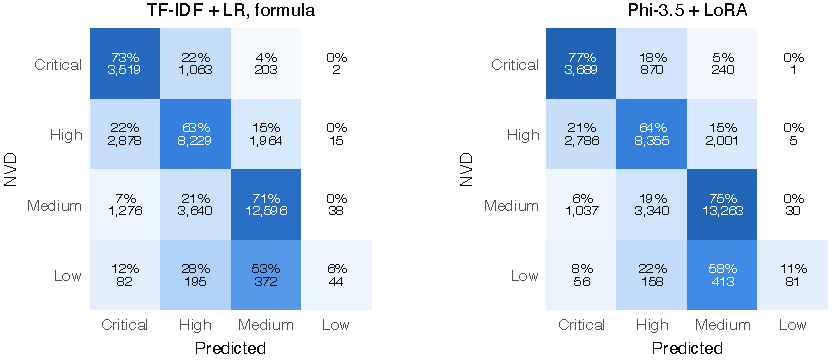
\includegraphics[width=\linewidth]{figures/fig_confusion.pdf}
\caption{Severity confusion matrices on the 2024 test set, normalized by true tier, for TF-IDF logistic regression with formula scoring (left) and fine-tuned Phi-3.5 (right).}
\label{fig:confusion}
\end{figure}

\paragraph{CVSS components.}
Figure~\ref{fig:components} gives accuracy per component, and attack complexity, scope, attack vector, and user interaction exceed 90\% for both systems because descriptions usually state them outright.
Privileges required is the hardest component (\nLRfCompPR\% for TF-IDF and \nLoRAfCompPR\% for the fine-tuned model), followed by the impact components, and the fine-tuned model gains most on confidentiality (\nLRfCompC\% to \nLoRAfCompC\%), integrity (\nLRfCompI\% to \nLoRAfCompI\%), and privileges required, the components that depend least on surface keywords.
\citet{marchiori2025canllms} found that general-purpose LLMs fall behind embedding-based classifiers on the impact components, whereas after fine-tuning these components are among those on which the model gains most over TF-IDF.

\begin{figure}[t]
\centering
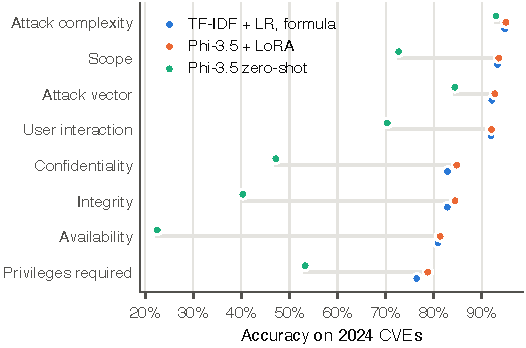
\includegraphics[width=0.62\linewidth]{figures/fig_components.pdf}
\caption{Accuracy per CVSS component on 2024 CVEs, with TF-IDF and the fine-tuned model scored on the full test set and the zero-shot model on its \nSub{}-CVE sample.}
\label{fig:components}
\end{figure}

\paragraph{Rare CWEs.}
The TF-IDF classifiers can output only the 100 most frequent training CWEs and therefore score 0\% on the \nRareCweN{} test CVEs whose CWE is rarer, whereas the fine-tuned model writes the CWE as text and identifies \nLoRAfRareCwe\% of them correctly (Figure~\ref{fig:cwe}), and common, explicitly named weaknesses such as cross-site scripting and SQL injection are close to solved by both systems.

\begin{figure}[t]
\centering
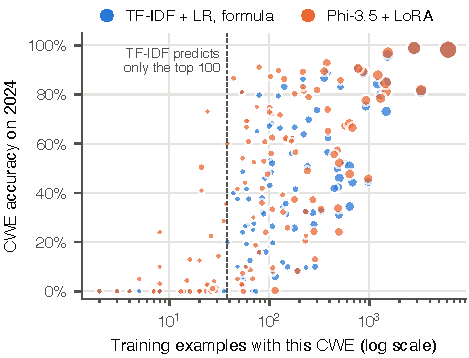
\includegraphics[width=0.62\linewidth]{figures/fig_cwe_frequency.pdf}
\caption{CWE accuracy on the 2024 test set against the number of training examples with each CWE, for every CWE with at least 20 test CVEs and with point size growing with test count.}
\label{fig:cwe}
\end{figure}

\paragraph{Score distribution.}
Ridge regression produces a smooth spread of scores that NVD never assigns and rarely predicts the extremes (Figure~\ref{fig:scores}), whereas the scores of the fine-tuned model sit on the same discrete values as those of NVD, although it predicts the most common critical score of 9.8 for \nLoRAfNineEight\% of test CVEs where NVD assigns it to \nNvdNineEight\%.
The fine-tuned model predicts \textsc{Critical} for \nLoRAfCritPred{} test CVEs against \nLoRAfCritTrue{} in NVD, with \nLoRAfCritPrec\% precision, and like formula-scored logistic regression it scores high on average, with a mean signed error of \nLoRAfBias.

\begin{figure}[t]
\centering
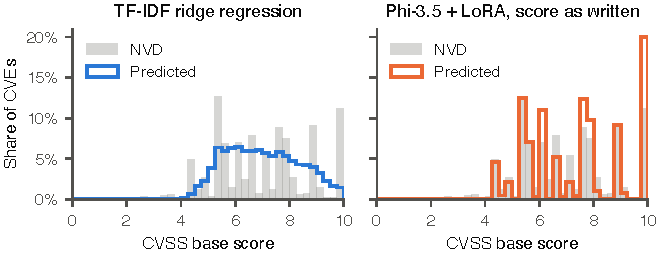
\includegraphics[width=0.75\linewidth]{figures/fig_score_dist.pdf}
\caption{Distribution of predicted and NVD base scores on the 2024 test set in bins of 0.25, for ridge regression (left) and the fine-tuned model with scores as written (right).}
\label{fig:scores}
\end{figure}

\subsection{Zero-Shot Baseline}
\begin{table}[t]
\centering
\caption{Comparison on the same random sample of 2{,}000 test CVEs, on which every system is scored.}
\label{tab:subset}
\small
\setlength{\tabcolsep}{4pt}
\begin{tabular}{lcccccc}
\toprule
 & \multicolumn{2}{c}{Severity} & CWE & Score & \multicolumn{2}{c}{Vector} \\
\cmidrule(lr){2-3}\cmidrule(lr){6-7}
System & Acc. & Macro-F1 & Acc. & MAE $\downarrow$ & Partial & Exact \\
\midrule
TF-IDF + LR, formula & 65.3\,{\scriptsize$\pm$2.1} & 47.6\,{\scriptsize$\pm$1.8} & 66.2\,{\scriptsize$\pm$2.2} & 0.99\,{\scriptsize$\pm$0.06} & 86.5\,{\scriptsize$\pm$0.7} & 42.2\,{\scriptsize$\pm$2.2} \\
Phi-3.5 zero-shot, direct & 20.8\,{\scriptsize$\pm$1.7} & 15.4\,{\scriptsize$\pm$2.4} & 25.7\,{\scriptsize$\pm$2.0} & 1.58\,{\scriptsize$\pm$0.05} & 60.5\,{\scriptsize$\pm$0.7} & 2.4\,{\scriptsize$\pm$0.6} \\
Phi-3.5 zero-shot, formula & 43.5\,{\scriptsize$\pm$2.3} & 26.8\,{\scriptsize$\pm$1.7} & 25.7\,{\scriptsize$\pm$2.0} & 2.08\,{\scriptsize$\pm$0.08} & 60.5\,{\scriptsize$\pm$0.7} & 2.4\,{\scriptsize$\pm$0.6} \\
Phi-3.5 + LoRA, formula & \textbf{69.6}\,{\scriptsize$\pm$2.0} & \textbf{52.8}\,{\scriptsize$\pm$3.3} & \textbf{68.8}\,{\scriptsize$\pm$2.1} & \textbf{0.87}\,{\scriptsize$\pm$0.05} & \textbf{87.5}\,{\scriptsize$\pm$0.7} & \textbf{48.0}\,{\scriptsize$\pm$2.1} \\
\bottomrule
\end{tabular}
\end{table}

Without fine-tuning, the same base model is far weaker (Table~\ref{tab:subset}), and although it returned valid JSON for \nZSParse\% of \nSub{} random test CVEs, the severity it writes is biased upward.
It labels \nZSCritShare\% of them \textsc{Critical} against \nSubCritShare\% in NVD and predicts \textsc{Medium} only \nZSMediumCount{} times although \nSubMediumShare\% of these CVEs are \textsc{Medium}, so its written severity is correct on only \nZSdSev\% of CVEs.
Its outputs also contradict themselves, since the score it writes matches the formula for its own vector on only \nZSScoreCons\% of CVEs and the severity it writes matches its own score on \nZSSevCons\% (Table~\ref{tab:consistency}).
Computing severity from its vector removes this inconsistency and raises severity accuracy to \nZSfSev\%, which remains well below the fine-tuned model (\nLoRAfSubSev\%) and TF-IDF (\nLRfSubSev\%) on the same CVEs.
Its score MAE, however, worsens from \nZSdMae{} to \nZSfMae{} because its vectors are often wrong in ways that move the score substantially, so for a zero-shot model formula scoring acts primarily as a consistency fix.

\begin{table}[htbp]
\centering
\caption{Self-consistency of language-model outputs (\%), where \emph{Score = formula} is the share of outputs whose written score equals the CVSS v3.1 score of the written vector and \emph{Severity = tier of score} is the share whose written severity matches the tier of the written score.}
\label{tab:consistency}
\small
\begin{tabular}{lccc}
\toprule
Model & Valid JSON & Score = formula & Severity = tier of score \\
\midrule
Phi-3.5 zero-shot & 99.7 & 3.4 & 37.0 \\
Phi-3.5 + LoRA & 100.0 & 99.8 & 100.0 \\
\bottomrule
\end{tabular}
\end{table}


\subsection{Training and Inference Cost}
Validation accuracy rose at every checkpoint, and the last checkpoint (step \nBestStep) was the best (Figure~\ref{fig:val}), which suggests that a further epoch might improve results.
\begin{table}[htbp]
\centering
\caption{Wall-clock time on a single Apple M5 Pro (64\,GB), with inference run in small batches of at most 32 CVEs and without optimization for speed.}
\label{tab:compute}
\small
\begin{tabular}{lr}
\toprule
Step & Time \\
\midrule
All TF-IDF baselines, tuning and test (CPU) & 9 min \\
LoRA fine-tuning, 5{,}000 steps & 2.5 h \\
LoRA inference, 36{,}325 test CVEs & 4.9 h \\
\bottomrule
\end{tabular}
\end{table}

Table~\ref{tab:compute} gives wall-clock times, with fine-tuning taking \nLoraTrainHours{} hours and scoring the full test year \nLoraTestHours{} hours, compared with \nTfidfMinutes{} minutes for all TF-IDF baselines together.

\begin{figure}[t]
\centering
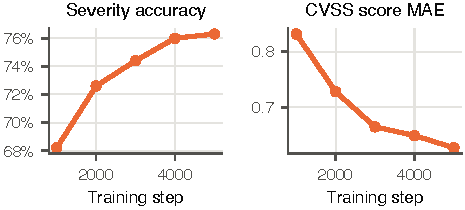
\includegraphics[width=0.55\linewidth]{figures/fig_val_curve.pdf}
\caption{Validation metrics of the fine-tuned model with formula scoring at each saved checkpoint, on 1,000 validation CVEs.}
\label{fig:val}
\end{figure}
